%%%%%%%%%%%%%%%%%%%%%%%%%%%%%%%%%%%%%%%%%%%%%%
%                insertmeeting
% 1) Title (something creative & funny?)
% 2) Date (MM/DD/YYYY)
% 3) Location (ex. Hagerty High School)
% 4) People/Committees Present 
% 5) Picture 
% 6) Start Time & Stop Time (ex. 12:30AM to 4:30PM)
%%%%%%%%%%%%%%%%%%%%%%%%%%%%%%%%%%%%%%%%%%%%%%
\insertmeeting 
	{Let's Orient Some Objects} 
	{01/13/22} 
	{Hagerty High School}
	{Annika, Anouska, Clayton, Falon, James, Jensen, Nathan, Ritam, Rose, Samantha, Lilly}
	{Images/RobotPics/robot.jpg}
	{2:30 - 4:30}
	
\hhscommittee{Software}
\noindent\hfil\rule{\textwidth}{.4pt}\hfil
\subsubsection*{Goals}
\begin{itemize}
    \item Implement our Road Runner classes into our robot's existing even-driven system. 

\end{itemize} 

\noindent\hfil\rule{\textwidth}{.4pt}\hfil

\subsubsection*{Accomplishments}
For today's extra long meeting, our goal was to create a class titled "TricycleRRDrive" that would mesh into our event-driven framework and the new localization methods we coded. The kinematic equations and localization processes are detailed in notebook entries over the last few days. 
To do this, we created a big method called "update" in the TricycleRRDrive class. This method will run every cycle and will handle our main logic. We created three states - IDLE, TURN, and FOLLOW TRAJECTORY that will each be called based on the robot's current task. TURN calculates the angle our robot should turn then uses the DriveSignal function we fixed a while ago to send power to the motors. Follow Trajectory takes the trajectory that we constructed and runs the robot along the path. Like before, it uses the DriveSignal function we created earlier. You'll also see some calls to the FtcDashboard. We've been running into some problems when combining Dashboard with our newer camera code, so the code doesn't work. However, we're confident that troubleshooting the errors caused by the camera will allow the dashboard to draw out our road runner paths. 
After that, we had to add the helper functions. The most important one is "driveSpline", allowing us to input a field coordinate and have the robot drive to it, automatically calculating road runner splines. It takes into account the direction we want the robot to travel and any constraints for the velocity. After we build the trajectory, the robot should go into the FOLLOW TRAJECTORY class. We simply send the power to the our existing drivebase class to make the robot move. Everything else we created (Kinematics, localization, and odometry) are working behind the scenes to keep everything updated. This feeds Road Runner accurate information to use. 
Thanks to Mr. Harper's help, we got the class running consistently. This project can be considered "complete" allowing us to move on to improving other parts of the robot. 
 
\begin{figure}[ht]
\centering
\begin{minipage}[b]{.48\textwidth}
  \centering
  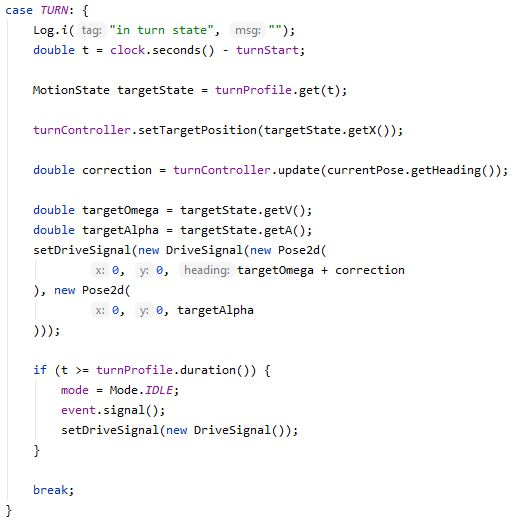
\includegraphics[width=0.95\textwidth]{Meetings/January/01-13-22/1-13-22 pic1 - James Hu.JPG}
  \caption{The TURN state}
  \label{fig:011322_1}
\end{minipage}%
\hfill%
\begin{minipage}[b]{.48\textwidth}
  \centering
  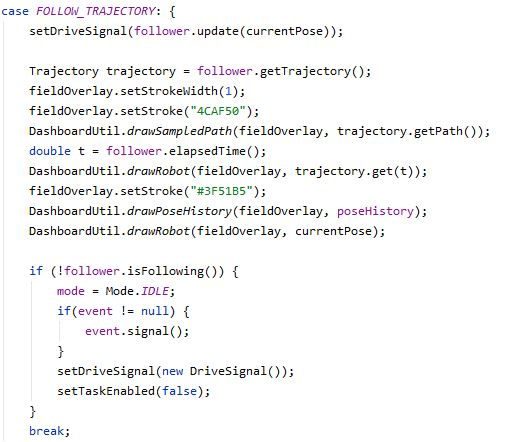
\includegraphics[width=0.95\textwidth]{Meetings/January/01-13-22/1-13-22 pic2 - James Hu.JPG}
  \caption{The TRAJECTORY state}
  \label{fig:011322_2}
\end{minipage}
\end{figure}

\begin{figure}[ht]
\centering
\begin{minipage}[b]{.48\textwidth}
  \centering
  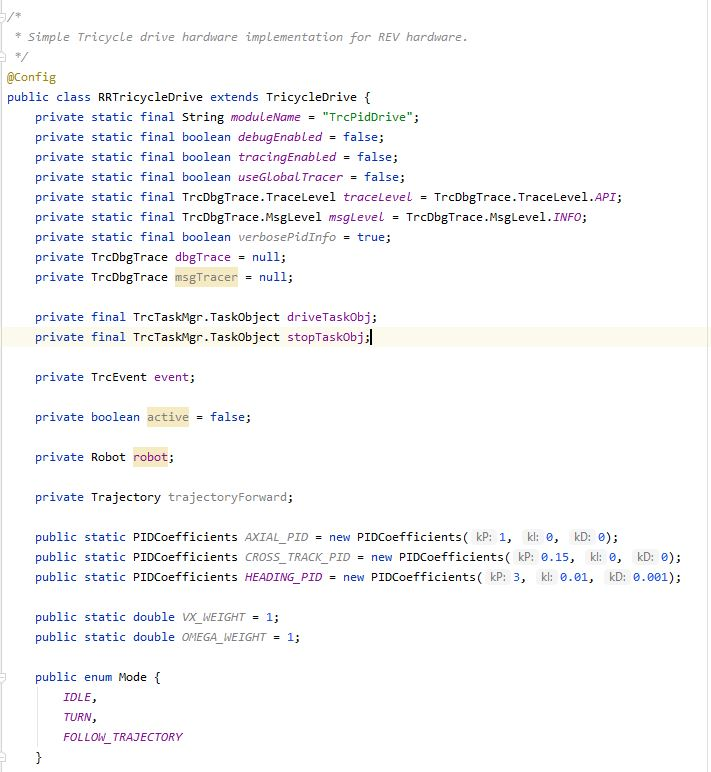
\includegraphics[width=0.95\textwidth]{Meetings/January/01-13-22/1-13-22 pic3 - James Hu.JPG}
  \caption{Our specific RRTricycleDrive extends the basic TricycleDrive class we created}
  \label{fig:011322_3}
\end{minipage}%
\hfill%
\begin{minipage}[b]{.48\textwidth}
  \centering
  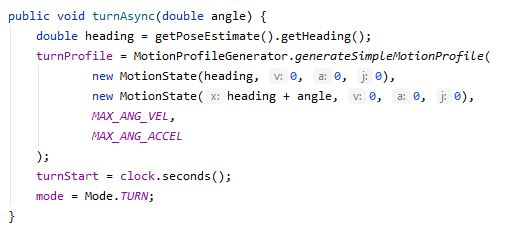
\includegraphics[width=0.95\textwidth]{Meetings/January/01-13-22/1-13-22 pic4 - James Hu.JPG}
  \caption{Our method to turn the robot using kinematics}
  \label{fig:011322_4}
\end{minipage}
\end{figure}


\begin{figure}[htp]
\centering
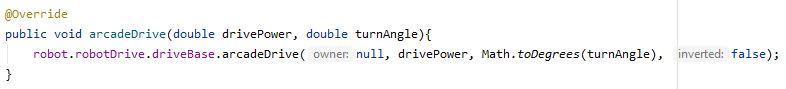
\includegraphics[width=0.95\textwidth, angle=0]{Meetings/January/01-13-22/1-13-22 pic5 - James Hu.JPG}
\caption{The way we connect our calculations class (RRTricycleDrive) to actual movement (HhsTricycleDrivebase)}
\label{fig:011322_5}
\end{figure}

\begin{figure}[htp]
\centering
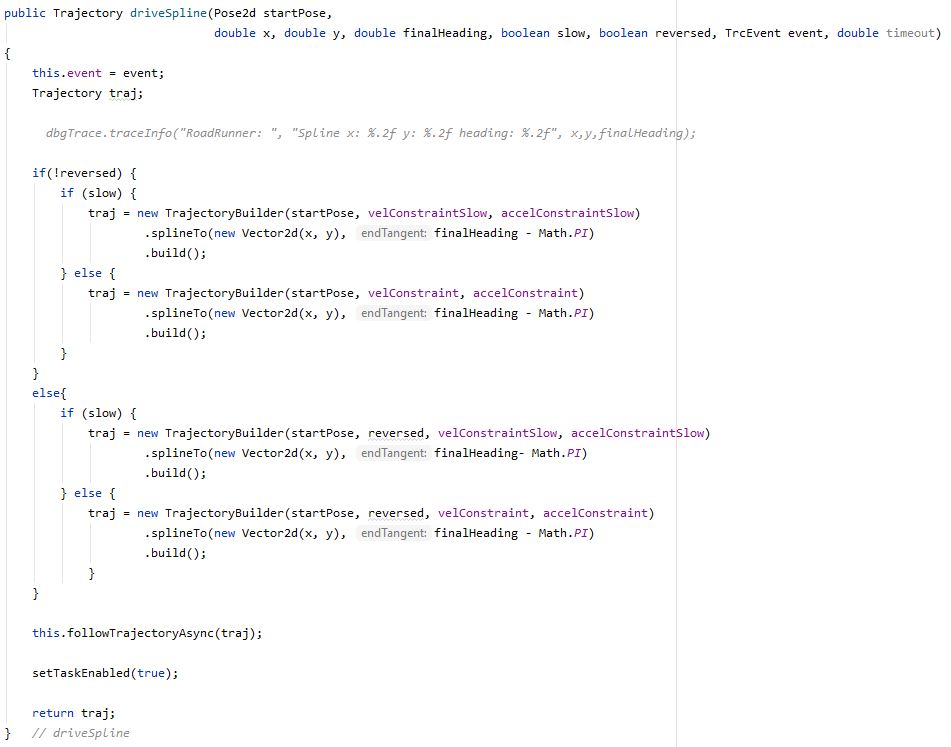
\includegraphics[width=0.95\textwidth, angle=0]{Meetings/January/01-13-22/1-13-22 pic6 - James Hu.JPG}
\caption{Our important method to build and follow spline curves}
\label{fig:011322_6}
\end{figure}





\whatsnext{
\begin{itemize}
    \item Finish commenting the class
	\item Move on to more camera work and fixing autonomous

\end{itemize} 
}

